\appendix

\section{Contributions}
\label{sec:contributions}

\textbf{\Acronym{} system design and implementation}: Pranav Atreya, Karl Pertsch, Tony Lee

\textbf{Experiment design and analysis}: Pranav Atreya, Karl Pertsch, Tony Lee

\textbf{Policy evaluation}: Pranav Atreya, Tony Lee, Moo Jin Kim, Karl Pertsch, Arhan Jain, Artur Kuramshin, Cyrus Neary, Edward Hu, Kanav Arora, Kirsty Ellis, Luca Macesanu, Matthew Leonard, Meedeum Cho, Ozgur Aslan, Shivin Dass, Jie Wang, William Reger, Xingfang Yuan

\textbf{Simulated evaluation environments}: Arhan Jain, Karl Pertsch, Xuning Yang, Clemens Eppner, Fabio Ramos, Jonathan Tremblay

\textbf{Paper writing}: Karl Pertsch, Pranav Atreya, Tony Lee

\textbf{Project coordination}: Karl Pertsch, Pranav Atreya

\textbf{Advising}: Sergey Levine, Chelsea Finn, Percy Liang, Abhishek Gupta, Dinesh Jayaraman, Glen Berseth, Kostas Daniilidis, Roberto Martin-Martin, Youngwoon Lee


\section{Policy Ranking EM Procedure}
\label{app:ranking_model}


Here we give additional details on our proposed policy ranking algorithm, introduced in section~\ref{sec:policy_ranking}. We first describe the underlying probabilistic model, derive all necessary gradients and Hessians, then present the complete EM pseudocode.  We then show how the algorithm can be easily modified to also use partial-success information when present, outline the algorithms behind the other ranking procedures discussed in the paper, and then list all hyperparameters.

\subsection{Model Definition}
\label{app:model_definition}

\paragraph{Observed data.}  
We assume a fixed set of \(N\) policies
\[
  \Pi = \{\pi_1,\pi_2,\dots,\pi_N\}.
\]
Evaluators compare policies in A/B trials: in trial \(n\), they pit policy
\(\pi_{i_n}\) against \(\pi_{j_n}\) on some (latent) task and report an outcome
\[
  y_n \;\in\;\{0,1,2\},
  \quad
  0=\text{loss},\;1=\text{tie},\;2=\text{win},
  \quad
  n=1,\dots,M.
\]
(Note this is a generalization of the model described in section~\ref{sec:policy_ranking}, which did not allow for ties.) We collect all \(M\) observations into
\[
  \mathcal{D}_p
  =\bigl\{\,\bigl(i_n,j_n,y_n\bigr)\bigr\}_{n=1}^M.
\]
At no point do we assume the true “task” identifiers are observed; instead we infer a small number of latent “task‐buckets” that capture varying difficulty levels.

\paragraph{Latent tasks and mixture weights.}  
To model varying evaluation conditions, we assume each trial belongs—unobserved—to one of \(T\) difficulty categories, or “buckets.”  We place a discrete prior over these buckets,
\[
  \nu = (\nu_1,\dots,\nu_T),
  \quad
  \nu_t \ge 0,\;\;\sum_{t=1}^T \nu_t = 1,
\]
so that before seeing any data, the probability a random trial uses bucket \(t\) is \(\nu_t\).

\paragraph{Per‐policy and per‐bucket parameters.}  
Each policy \(\pi_p\) has a global “log‐ability” parameter \(\theta_p\).  Additionally, each policy may perform better or worse on certain buckets, so we introduce an offset \(\psi_{p,t}\) for policy \(p\) on bucket \(t\). This offset serves the purpose of enabling two policies to perform differently relative to each other on different tasks (the motivation for the introduction of this offset is discussed further in section~\ref{sec:policy_ranking}). Finally, each bucket \(t\) has a base difficulty \(\tau_t\).  Collecting these,
\[
  \theta = (\theta_1,\dots,\theta_N),\quad
  \psi = \{\psi_{p,t}\}_{p=1..N,\;t=1..T},\quad
  \tau = (\tau_1,\dots,\tau_T).
\]
Intuitively, \(\theta_p\) captures overall policy strength, \(\tau_t\) captures bucket difficulty, and \(\psi_{p,t}\) models policy‐specific ease or difficulty adjustments within each bucket.

\paragraph{Tie‐model parameter.}  
We allow ties via the Davidson extension, introducing a single scalar \(\nu_{\rm tie}\in(0,1)\) which scales the draw probability relative to wins and losses.

\paragraph{Link function and conditional likelihood.}  
Given trial \(n\) and hypothesized bucket \(t\), compute each policy’s log‐odds,
\[
  z_{i_n,t}
    = \theta_{i_n} + \psi_{i_n,t} - \tau_t,
  \quad
  z_{j_n,t}
    = \theta_{j_n} + \psi_{j_n,t} - \tau_t.
\]
Pass these through the logistic sigmoid (our instantiation of the \emph{link-function}, which generally is a mapping from linear predictors, here our log-odds, to probabilities) \(\sigma(z)=1/(1+e^{-z})\) to get
\[
  q_{i_n,t} = \sigma(z_{i_n,t}),
  \quad
  q_{j_n,t} = \sigma(z_{j_n,t}).
\]
Under the “independent‐solve” assumption, policy \(i_n\) “solves” the task with probability \(q_{i_n,t}\) and \(j_n\) with probability \(q_{j_n,t}\), independently given \(t\).  Even though our dataset represents preferences between policies $i$ and $j$, this “independent‐solve” assumption is natural because in actuality, the performance of policy $i$ on the task is independent to that of policy $j$. Thus
\[
  P(y_n=2\mid t)
    = q_{i_n,t}\,\bigl(1 - q_{j_n,t}\bigr),
  \quad
  P(y_n=0\mid t)
    = \bigl(1 - q_{i_n,t}\bigr)\,q_{j_n,t},
\]
\[
  P(y_n=1\mid t)
    = 2\,\nu_{\rm tie}\,
      \sqrt{q_{i_n,t}(1 - q_{i_n,t})\,q_{j_n,t}(1 - q_{j_n,t})}\,,
\]
again invoking the Davidson extension of the Bradley-Terry model. Because \(t\) is latent, we marginalize over buckets:
\[
  P(y_n)
   = \sum_{t=1}^{T} \nu_t \;P\!\bigl(y_n\mid t\bigr).
\]
This completes the model definition.


\subsection{Gradient \& Hessian Derivation}
\label{app:grad_hess}

Below we derive all first and second derivatives needed for the clipped‐Newton M‐step.  We begin by writing the expected complete‐data objective and then expand gradients and Hessians for each parameter block.

\paragraph{Expected complete‐data objective.}  
Denote the full parameter set by \(\Theta=(\theta,\psi,\tau,\nu,\nu_{\rm tie})\).  In the E–step we compute responsibilities
\[
  \gamma_{n,t}
  = P\bigl(t\mid y_n;\Theta^{\rm old}\bigr)
  = \frac{\nu_t\,P(y_n\mid t;\Theta^{\rm old})}
         {\sum_{u=1}^T \nu_u\,P(y_n\mid u;\Theta^{\rm old})}.
\]
The expected complete‐data log‐likelihood, including L2 penalties \(\lambda_\theta,\lambda_\psi\), is
\[
  Q(\Theta)
  = \sum_{n=1}^M\sum_{t=1}^T
      \gamma_{n,t}\,\Bigl[\log\nu_t + \log P(y_n\mid t)\Bigr]
    \;-\;\frac{\lambda_\theta}{2}\sum_{p=1}^N \theta_p^2
    \;-\;\frac{\lambda_\psi}{2}\sum_{p=1}^N\sum_{t=1}^T \psi_{p,t}^2.
\]

\paragraph{Gradient w.r.t.\ \(\theta_p\).}  
Only trials where policy \(p\) appears contribute.  Let
\(\mathcal{I}_p=\{n:i_n=p\}\), \(\mathcal{J}_p=\{n:j_n=p\}\).  Then
\[
  \frac{\partial Q}{\partial\theta_p}
  = \sum_{n\in\mathcal{I}_p}\sum_{t=1}^T
      \gamma_{n,t}\,\frac{\partial}{\partial z_{i_n,t}}
      \log P(y_n\mid t)
  - \sum_{n\in\mathcal{J}_p}\sum_{t=1}^T
      \gamma_{n,t}\,\frac{\partial}{\partial z_{j_n,t}}
      \log P(y_n\mid t)
  - \lambda_\theta\,\theta_p.
\]
For instance, for \(y_n=2\) (a “win”), one finds
\[
  \frac{\partial}{\partial z_{i,t}}\log P(y_n=2\mid t)
    = 1 - \sigma(z_{i,t}),
  \qquad
  \frac{\partial}{\partial z_{j,t}}\log P(y_n=2\mid t)
    = -\,\sigma(z_{j,t}),
\]
with analogous expressions in the loss or tie case.

\paragraph{Hessian w.r.t.\ \(\theta_p\).}  
The second derivative accumulates the negative of the logistic variances:
\[
  \frac{\partial^2 Q}{\partial\theta_p^2}
  = -\,\sum_{n\in\mathcal{I}_p}\sum_t
      \gamma_{n,t}\,\sigma(z_{i,t})(1-\sigma(z_{i,t}))
    -\sum_{n\in\mathcal{J}_p}\sum_t
      \gamma_{n,t}\,\sigma(z_{j,t})(1-\sigma(z_{j,t}))
    - \lambda_\theta.
\]

\paragraph{Gradients/Hessians for \(\psi_{p,t}\).}  
Each \(\psi_{p,t}\) enters exactly like \(\theta_p\) but only for bucket \(t\):
\[
  \frac{\partial Q}{\partial\psi_{p,t}}
  = \sum_{n:i_n=p}\gamma_{n,t}\,\frac{\partial\log P}{\partial z_{i_n,t}}
  - \sum_{n:j_n=p}\gamma_{n,t}\,\frac{\partial\log P}{\partial z_{j_n,t}}
  - \lambda_\psi\,\psi_{p,t},
\]
\[
  \frac{\partial^2Q}{\partial\psi_{p,t}^2}
  = -\sum_{n:i_n=p}\gamma_{n,t}\,\sigma(z_{i,t})(1-\sigma(z_{i,t}))
    -\sum_{n:j_n=p}\gamma_{n,t}\,\sigma(z_{j,t})(1-\sigma(z_{j,t}))
    - \lambda_\psi.
\]

\paragraph{Gradients/Hessians for \(\tau_t\).}  
Since \(\tau_t\) enters with a minus sign in both \(i\) and \(j\),
\[
  \frac{\partial Q}{\partial\tau_t}
  = -\sum_{n=1}^M \gamma_{n,t}\,\Bigl[
      \tfrac{\partial}{\partial z_{i,t}}\log P(y_n\mid t)
    + \tfrac{\partial}{\partial z_{j,t}}\log P(y_n\mid t)
    \Bigr],
\]
\[
  \frac{\partial^2Q}{\partial\tau_t^2}
  = -\sum_{n=1}^M \gamma_{n,t}\,\Bigl[
      \sigma(z_{i,t})(1-\sigma(z_{i,t}))
    + \sigma(z_{j,t})(1-\sigma(z_{j,t}))
    \Bigr].
\]

All of these gradient and Hessian terms are used in the M‐step clipped‐Newton updates described in Algorithm~\ref{alg:hybrid-em-full}.

\begin{algorithm}[ht]
\caption{EM for Fitting Model Parameters}
\label{alg:hybrid-em-full}
\begin{algorithmic}[1]
\Require Data $\{(i_n,j_n,y_n)\}_{n=1}^M$, number of buckets $T$, max iters \textsf{EM\_ITERS}
\Ensure $\theta,\;\psi,\;\tau,\;\nu,\;\nu_{\rm tie}$ and sorted policy ranking
\State {\bf Initialize:}
\State\quad $\theta_p\sim\mathcal N(0,0.1)$ for $p=1,\dots,N$
\State\quad $\psi_{p,t}\gets0$ for all $p,t$
\State\quad $\tau_t\sim\mathcal N(0,0.1)$ for $t=1,\dots,T$
\State\quad Mixture weights: $\nu_t\gets 1/T$ for $t=1,\dots,T$
\State\quad Tie‐parameter: $\nu_{\rm tie}\gets 0.5$
\For{$m=1$ \textbf{to} \,\textsf{EM\_ITERS}} \\
  \Comment{--- E–step: compute responsibilities ---}
  \For{$n=1$ \textbf{to} $M$}
    \State compute $P(y_n\mid t)$ for each bucket $t$
    \State $\gamma_{n,t}\gets \nu_t\,P(y_n\mid t)$
    \State normalize $\{\gamma_{n,1},\dots,\gamma_{n,T}\}$ so they sum to 1
  \EndFor

  \Comment{--- M–step: clipped‐Newton updates ---}
  \For{each policy $p=1,\dots,N$}
    \State compute gradient $g_p\!=\!\partial Q/\partial\theta_p$ and Hessian $h_p\!=\!\partial^2Q/\partial\theta_p^2$
    \State $\theta_p\gets \theta_p - \mathrm{clip}\bigl(g_p/h_p\bigr)$
  \EndFor

  \For{each $(p,t)$ with $p=1..N,\;t=1..T$}
    \State compute $g_{p,t}\!=\!\partial Q/\partial\psi_{p,t}$ and $h_{p,t}\!=\!\partial^2Q/\partial\psi_{p,t}^2$
    \State $\psi_{p,t}\gets \psi_{p,t} - \mathrm{clip}\bigl(g_{p,t}/h_{p,t}\bigr)$
  \EndFor

  \For{each bucket $t=1,\dots,T$}
    \State compute $g_t\!=\!\partial Q/\partial \tau_t$ and $h_t\!=\!\partial^2Q/\partial\tau_t^2$
    \State $\tau_t\gets \tau_t - \mathrm{clip}\bigl(g_t/h_t\bigr)$
  \EndFor

  \State {\bf Update mixture weights and tie‐rate:}
  \State\quad $\nu_t \gets \dfrac{1}{M}\sum_{n=1}^M \gamma_{n,t}$
  \State\quad $\nu_{\rm tie} \gets 0.5 \times \dfrac{\sum_{n,t}\gamma_{n,t}\,p_{\rm tie}(n,t)}{\sum_{n,t}\gamma_{n,t}\,p_{\rm win}(n,t)}$
  
  \If{maximum change in any $\theta_p$ $<\,$\textsf{tol}}
    \State \textbf{break}
  \EndIf
\EndFor

\State \Return policies sorted in descending order of $\theta_p$
\end{algorithmic}
\end{algorithm}

\subsection{Including Partial‐Success Information}

When available, the algorithm can be easily modified to make use of partial success information 
\(\,s^{(i)}_n, s^{(j)}_n\in[0,1]\).  We introduce an extra Gaussian term
\(\exp[-((s^{(i)}-q_i)^2+(s^{(j)}-q_j)^2)/(2\sigma_{\rm partial}^2)]^{w_{\rm ps}}\)
in the E–step likelihood and add its gradients/Hessians in the M–step exactly as in sections~\ref{app:model_definition} and~\ref{app:grad_hess}.  The modified pseudocode adds two lines in the E–step and augments each \(g,h\) with the partial‐success contributions.

\subsection{Baseline Ranking Algorithms}
\label{app:baselines}

Below we summarize the simpler ranking methods we compare against, including both classic preference‐only approaches and a simple partial‐success approach.

\paragraph{Bradley–Terry MLE (offline).}  
In the standard Bradley–Terry maximum‐likelihood estimator, we posit
\[
  P(y_n=2)\;=\;\sigma\bigl(\theta_{i_n}-\theta_{j_n}\bigr),
\]
and fit the ability parameters \(\theta\) by maximizing the log‐likelihood of all win/loss outcomes (ties can be handled via small modifications).  A simple gradient‐ascent update is
\[
  \theta_p \;\gets\;
    \theta_p \;+\;\eta
    \sum_{n:\,i_n=p}\Bigl[y_n - \sigma\bigl(\theta_{i_n}-\theta_{j_n}\bigr)\Bigr]
    \;-\;
    \eta
    \sum_{n:\,j_n=p}\Bigl[y_n - \sigma\bigl(\theta_{i_n}-\theta_{j_n}\bigr)\Bigr],
\]
where \(\eta\) is a small learning rate, \(y_n=2\) for a win by \(i_n\), \(y_n=0\) for a loss, and ties are typically treated as half-win/half-loss.  Iterating this update until convergence yields the offline MLE of the BT model.  In practice one also adds L2 regularization \(\lambda\theta_p\) to stabilize training.

\newpage

\paragraph{Elo‐style online update.}  
Elo is a one‐pass, online version of BT often used in rating chess players.  After each observed comparison between \(A\) and \(B\), one updates only the two involved ratings:
\[
  \theta_A \;\gets\;
    \theta_A \;+\; K\,\Bigl(y_{AB} - \sigma(\theta_A-\theta_B)\Bigr),
  \quad
  \theta_B \;\gets\;
    \theta_B \;-\; K\,\Bigl(y_{AB} - \sigma(\theta_A-\theta_B)\Bigr),
\]
where \(K\) is a constant “K‐factor,” and \(y_{AB}=1\) if \(A\) wins, \(0\) if \(A\) loses (ties set \(y_{AB}=0.5\)).  This update has the property of immediate rating adjustments as data arrives and requires no global passes over the dataset.

\paragraph{Partial‐Success Averaging.}  
As a non‐preference baseline, one can ignore all binary outcomes and instead rank policies by their \emph{average partial‐success rate} across all rollouts.  Concretely, if policy \(p\) receives a fractional success score \(s_{n}^{(p)}\in[0,1]\) on each trial \(n\), we compute
\[
  \bar s_p \;=\;
    \frac{1}{N_p}\sum_{n:\,i_n=p \text{ or } j_n=p}
      \bigl[s_{n}^{(p)}\bigr],
\]
where \(N_p\) is the total number of rollouts involving \(p\).  Finally, we sort policies in descending order of \(\bar s_p\).  This method leverages continuous performance feedback directly, but does not account for the paired‐comparison structure of A/B evaluations.

\subsection{Hyperparameter Table}

\begin{table}[H]
\centering
\begin{tabular}{lcc}
\toprule
Parameter              & Default           & Search range             \\
\midrule
EM\_ITERS              & 60               & $\{50,100,200\}$         \\
\# buckets $T$         & 60                 & $\{10...200\}$           \\
step\_clip             & 1.0               & $[0.1,\,10]$              \\
l2\_theta              & $10^{-2}$         & $\{10^{-3},10^{-2},10^{-1}\}$ \\
l2\_psi                & $10^{-2}$         & $\{10^{-3},10^{-2},10^{-1}\}$ \\
step\_decay            & 0.99              & $\{0.9,0.99,0.999\}$      \\
tol                    & $10^{-4}$         & $\{10^{-5},10^{-4}\}$     \\
\bottomrule
\end{tabular}
\caption{EM procedure hyperparameters.}
\end{table}

\subsection{Simulating Shifts in the Task Distribution and Policy Set}

The intent of the RoboArena platform is for it to serve as a long-running evaluation and benchmarking resource for the robotics community. In such a setting, it is likely that the policy set will evolve over time, with weaker policies getting dropped and stronger policies getting added to the pool. At the same time, as the capabilities of policies evolve, evaluators will likely adjust the tasks they set up for evaluation to better test the new policy capabilities. 

We test whether the RoboArena ranking model will remain valid and performant under distribution shifts over time. We rerun our rankings  with artificial drift in task difficulty (as judged by average per-task progress scores), starting with easy tasks and moving towards harder tasks over time, while at the same time phasing out weaker policies and adding stronger policies to the evaluation pool over time (again judged by per-policy progress scores). This simulates RoboArena’s development as a community benchmark with increasingly capable policies and increasingly challenging task distributions. The results in Table~\ref{tab:ranking_under_dist_shifts} show that even under these more challenging circumstances, RoboArena evaluations retain significantly higher correlation with oracle scores than “Regular” evaluations in a single laboratory.

\begin{table}[H]
\centering
\begin{tabular}{lcc}
\toprule
\textbf{Eval Approach}              & \textbf{Pearson} $r (\uparrow)$           & \textbf{MMRV} $(\downarrow)$             \\
\midrule
Regular              & 0.692               & 0.141         \\
RoboArena w/ dist. shifts (ours)         & \textbf{0.838}                 & \textbf{0.058}           \\
\bottomrule
\end{tabular}
\vspace{0.1cm}
\caption{RoboArena under simulated distribution shifts.}
\label{tab:ranking_under_dist_shifts}
\end{table}


\section{Evaluation Data Breakdown}
\label{app:detailed_eval_breakdown}


Here we depict in detail the evaluation data collected by RoboArena, emphasizing it's diversity and scale. To the best of our knowledge, the evaluations done thus far with RoboArena constitute the most comprehensive evaluations of generalist policies to date. 

Figure~\ref{fig:instruction_diversity} depicts on the top the diversity in the \emph{verb} making up the task command, and on the bottom the wide range of object classes that are being interacted with during the evaluation episodes. Generalist policies are uniquely data demanding when it comes to evaluations, as to properly assess a policy's performance as a generalist, the policy must be queried with a diverse array of tasks. Indeed, figure~\ref{fig:instruction_diversity} shows that the RoboArena evaluation procedure permits the required diversity in task commands and objects.
Figure~\ref{env_collage} similarly shows a representation of the diversity of RoboArena evaluations with respect to the set of scenes upon which evaluations were performed. The environments sampled were chosen randomly from the pool of all evaluation episodes.

\begin{figure}[H]
    \centering
    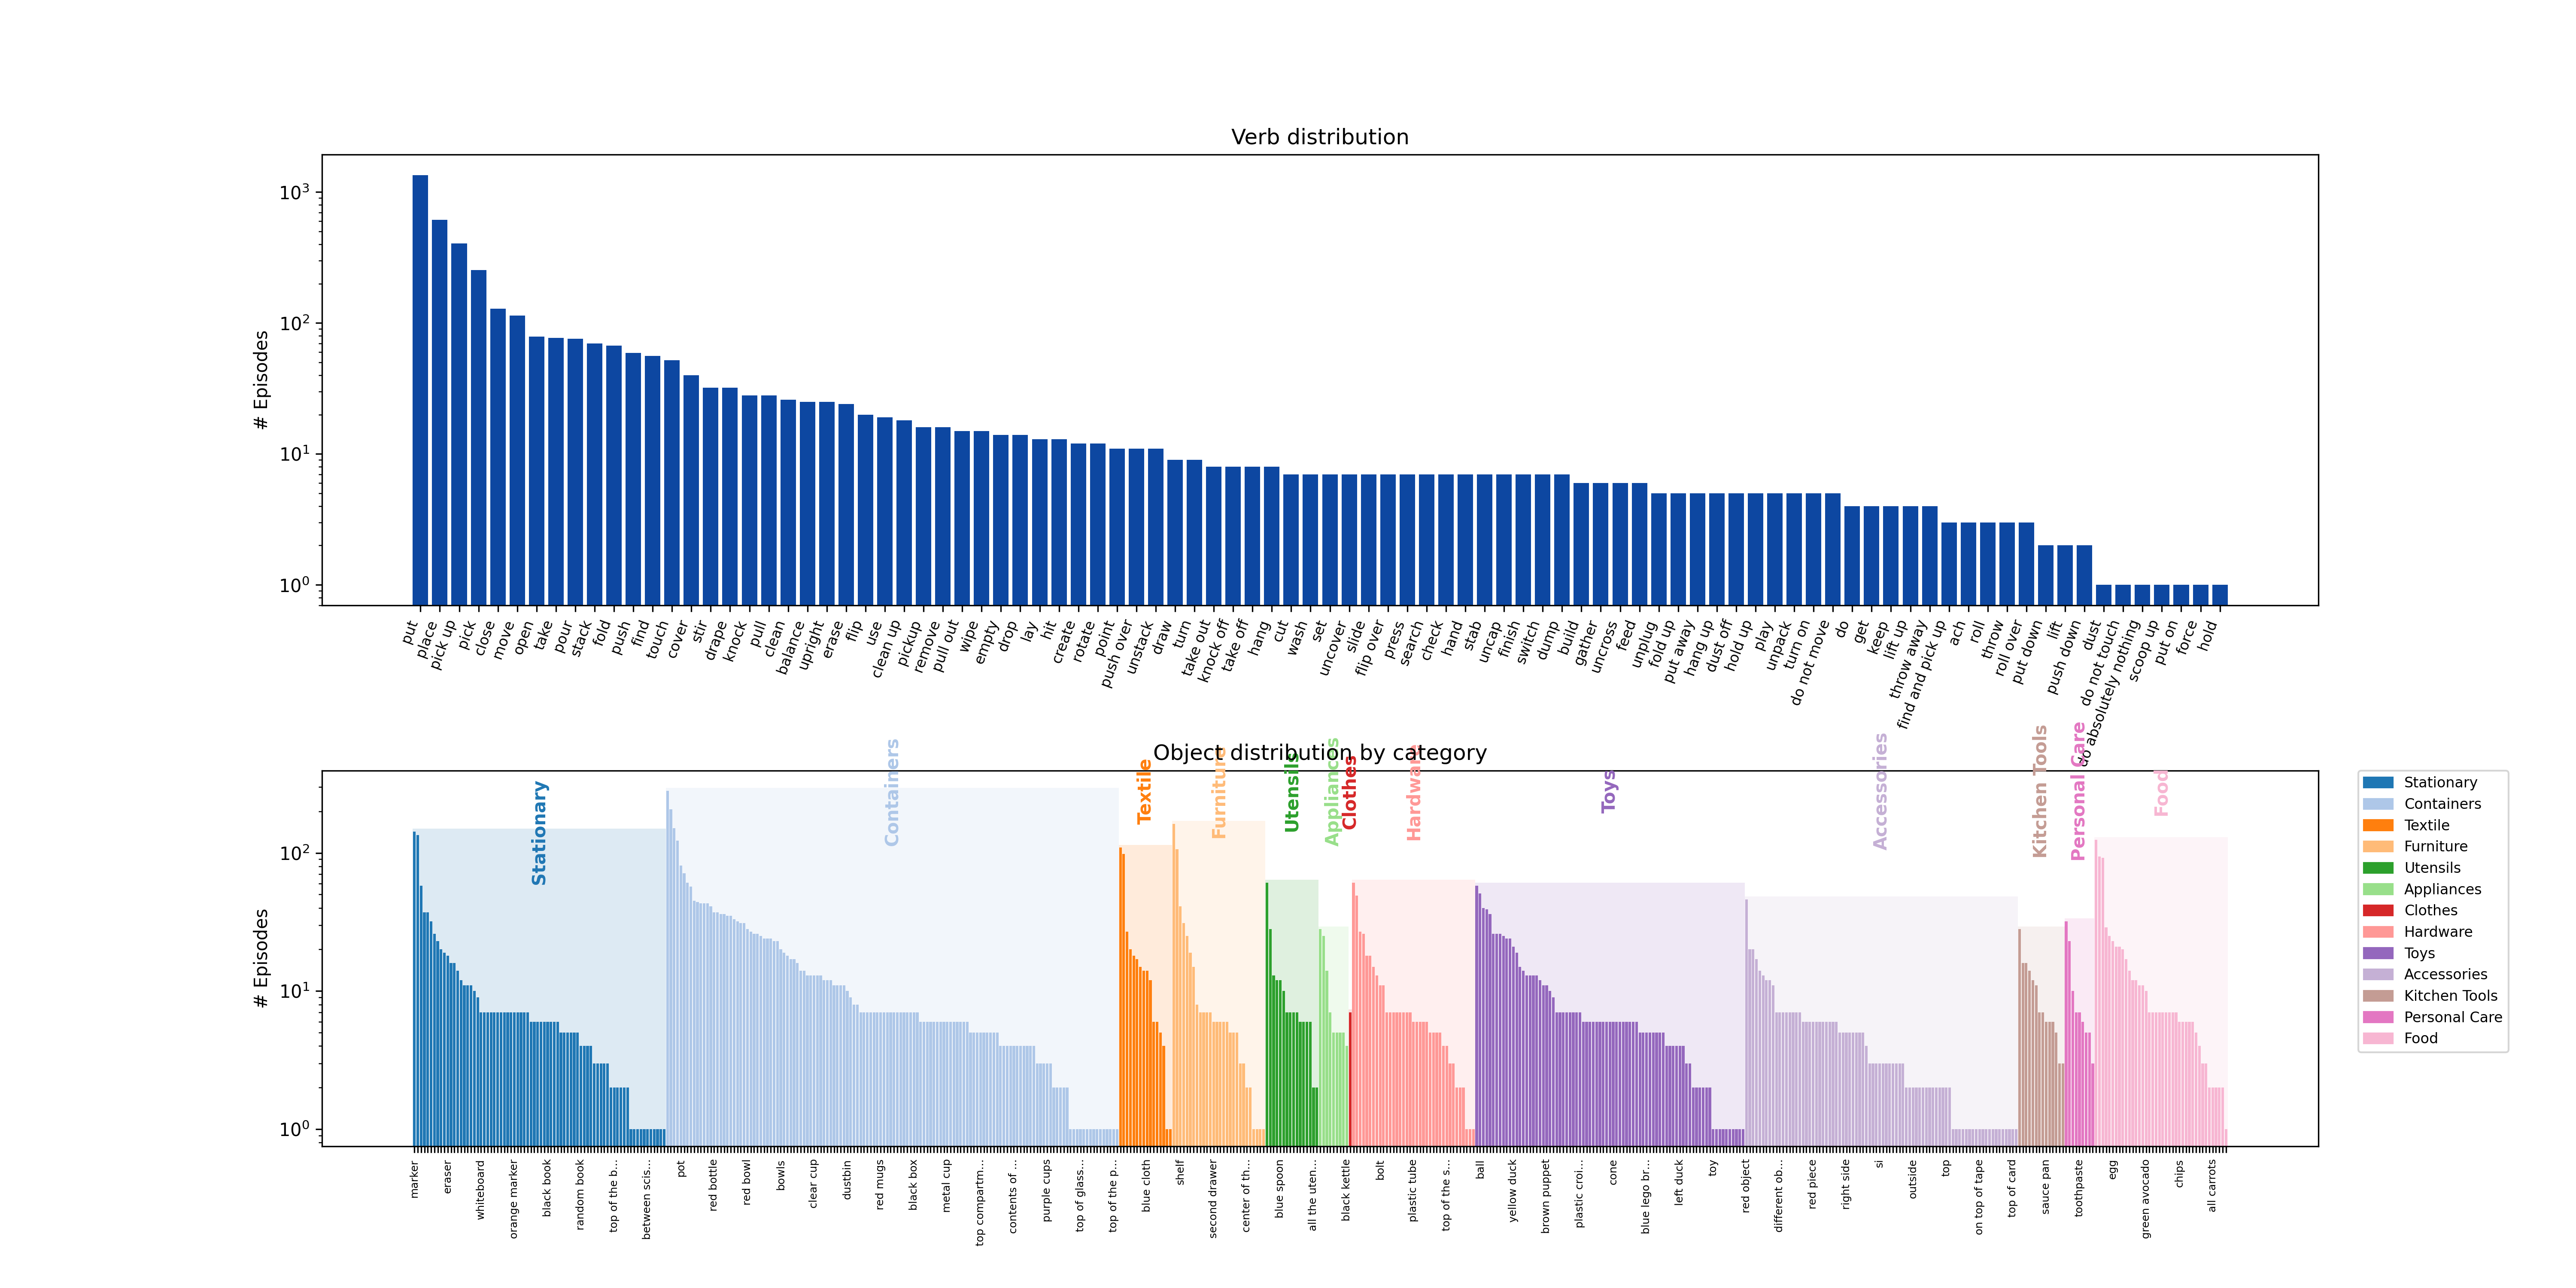
\includegraphics[width=\linewidth]{figures/instruction_diversity.png}
    \caption{\textbf{Top:} bar chart of the most common verbs used in the task commands, along with their frequencies in the evaluation data collected. The task commands exhibit a diverse array of instructions, including "uncapping", "unplugging", "finding", "dusting", etc. \textbf{Bottom:} visualization of the diversity of object categories being commanded to be interacted with, bucketed by major objects types.}
    \label{fig:instruction_diversity}
\end{figure}

\begin{figure}[H]
  \centering
  \setlength{\tabcolsep}{1pt}
  \renewcommand{\arraystretch}{0}
  \begin{tabular}{cccc}
    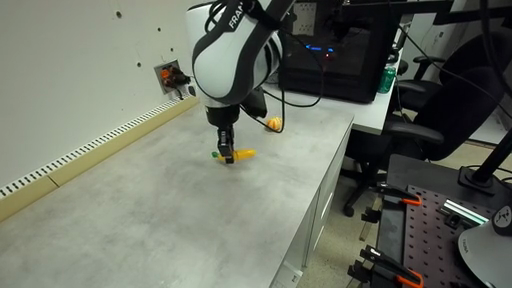
\includegraphics[width=0.23\textwidth]{figures/collage_of_envs/1.png}  &
    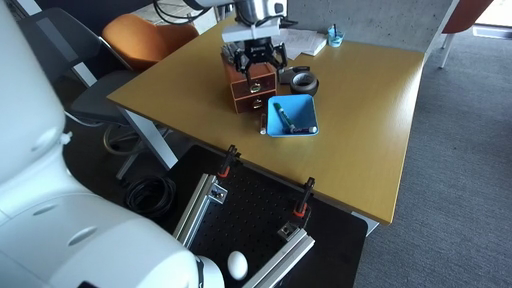
\includegraphics[width=0.23\textwidth]{figures/collage_of_envs/2.png}  &
    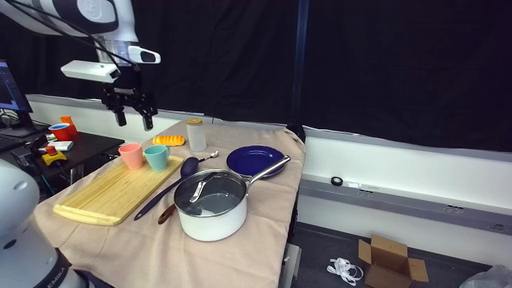
\includegraphics[width=0.23\textwidth]{figures/collage_of_envs/3.png}  &
    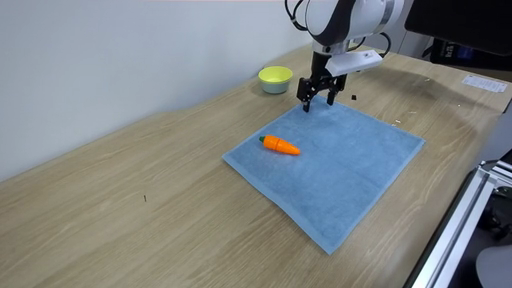
\includegraphics[width=0.23\textwidth]{figures/collage_of_envs/4.png}  \\[-2pt]
    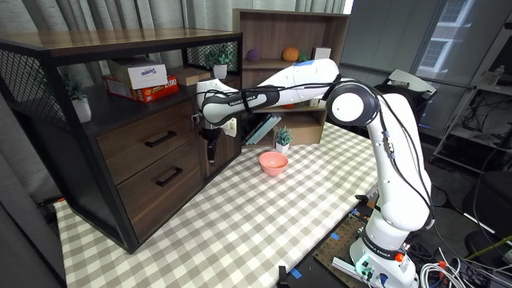
\includegraphics[width=0.23\textwidth]{figures/collage_of_envs/5.png}  &
    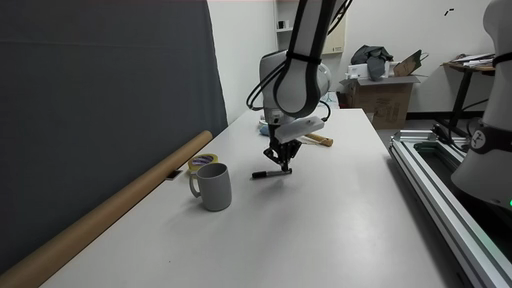
\includegraphics[width=0.23\textwidth]{figures/collage_of_envs/6.png}  &
    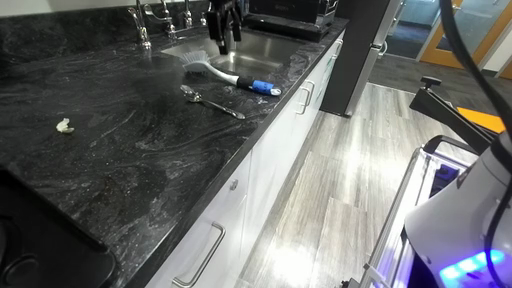
\includegraphics[width=0.23\textwidth]{figures/collage_of_envs/7.png}  &
    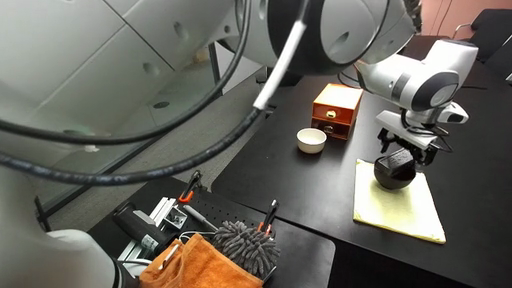
\includegraphics[width=0.23\textwidth]{figures/collage_of_envs/8.png}  \\[-2pt]
    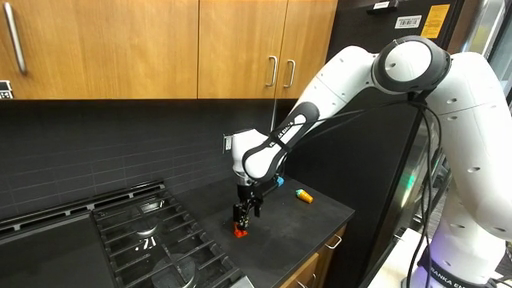
\includegraphics[width=0.23\textwidth]{figures/collage_of_envs/9.png}  &
    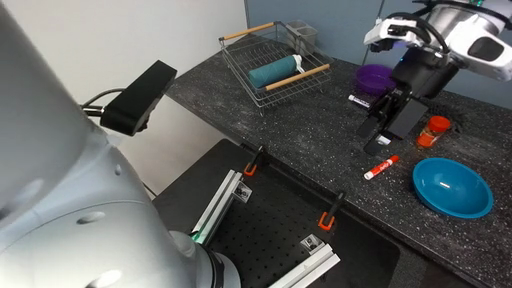
\includegraphics[width=0.23\textwidth]{figures/collage_of_envs/10.png} &
    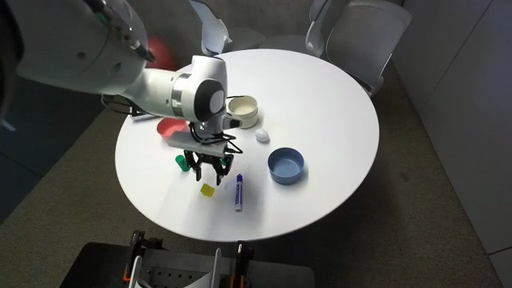
\includegraphics[width=0.23\textwidth]{figures/collage_of_envs/11.png} &
    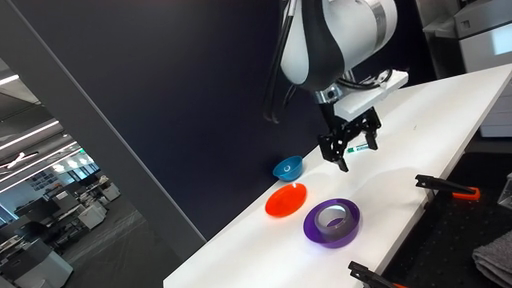
\includegraphics[width=0.23\textwidth]{figures/collage_of_envs/12.png} \\[-2pt]
    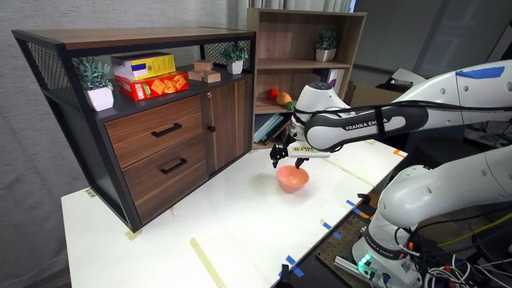
\includegraphics[width=0.23\textwidth]{figures/collage_of_envs/13.png} &
    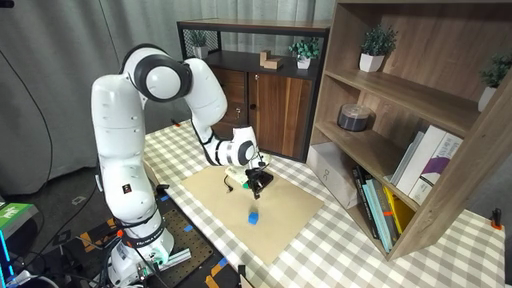
\includegraphics[width=0.23\textwidth]{figures/collage_of_envs/14.png} &
    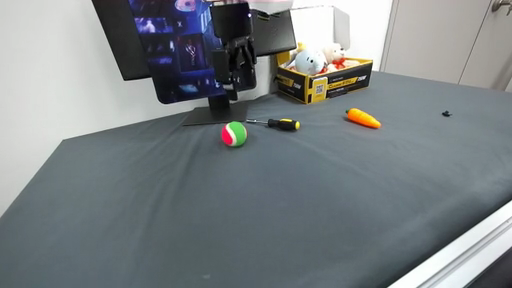
\includegraphics[width=0.23\textwidth]{figures/collage_of_envs/15.png} &
    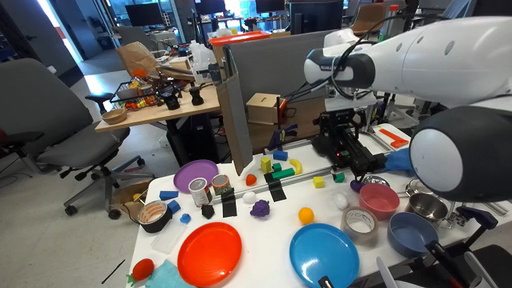
\includegraphics[width=0.23\textwidth]{figures/collage_of_envs/16.png} \\[-2pt]
    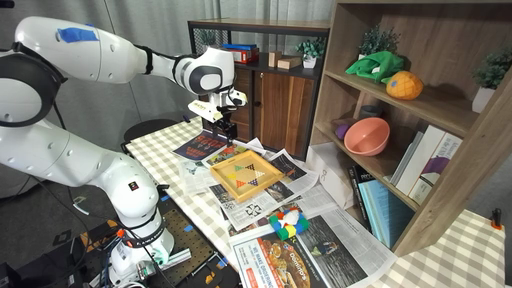
\includegraphics[width=0.23\textwidth]{figures/collage_of_envs/17.png} &
    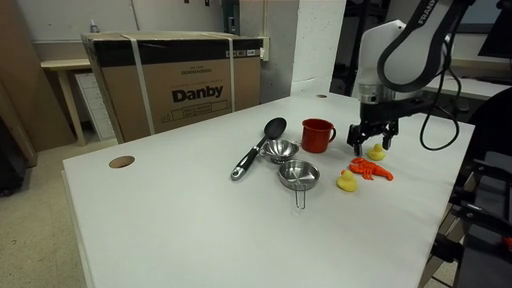
\includegraphics[width=0.23\textwidth]{figures/collage_of_envs/18.png} &
    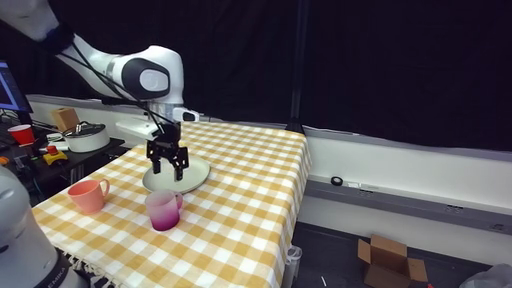
\includegraphics[width=0.23\textwidth]{figures/collage_of_envs/19.png} &
    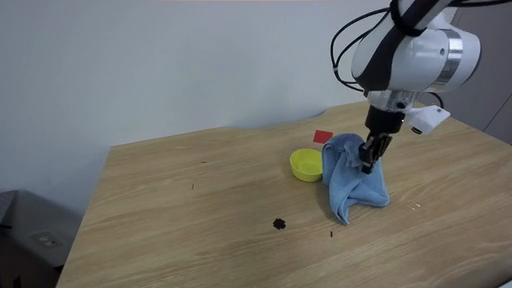
\includegraphics[width=0.23\textwidth]{figures/collage_of_envs/20.png} \\[-2pt]
    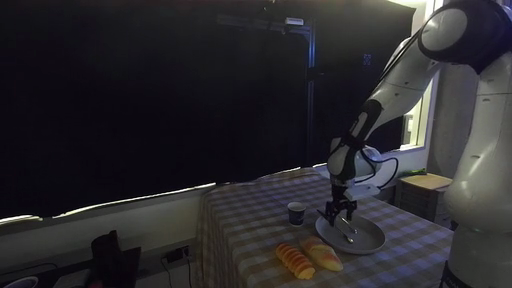
\includegraphics[width=0.23\textwidth]{figures/collage_of_envs/21.png} &
    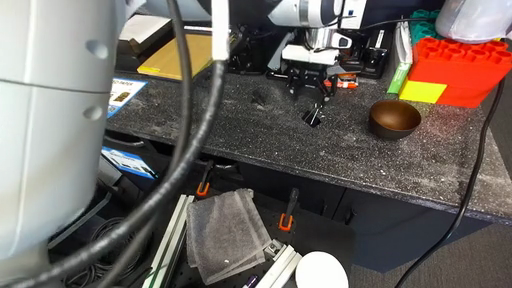
\includegraphics[width=0.23\textwidth]{figures/collage_of_envs/22.png} &
    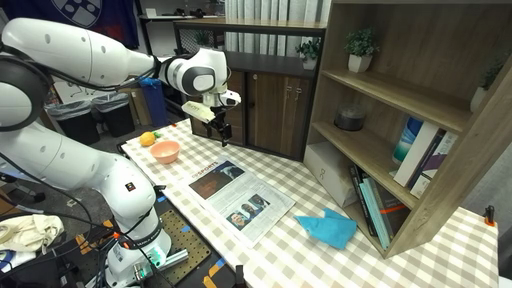
\includegraphics[width=0.23\textwidth]{figures/collage_of_envs/23.png} &
    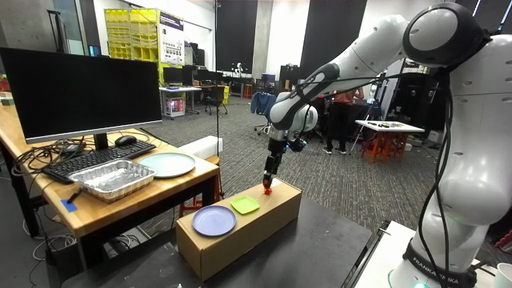
\includegraphics[width=0.23\textwidth]{figures/collage_of_envs/24.png} \\[-2pt]
    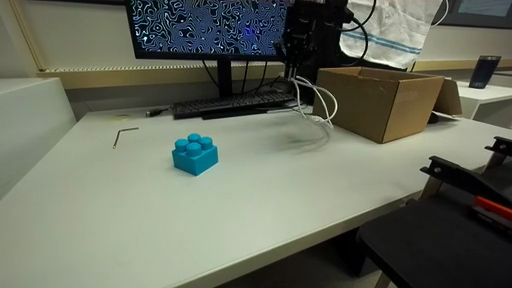
\includegraphics[width=0.23\textwidth]{figures/collage_of_envs/25.png} &
    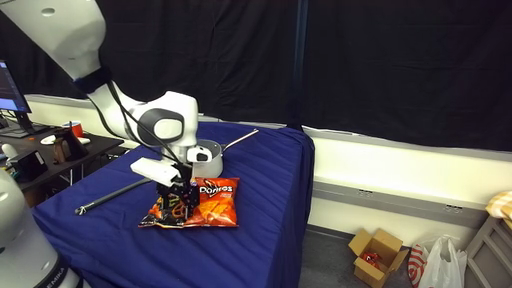
\includegraphics[width=0.23\textwidth]{figures/collage_of_envs/26.png} &
    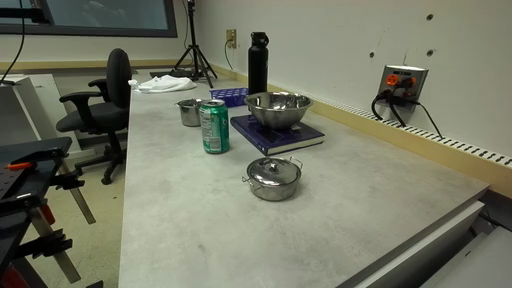
\includegraphics[width=0.23\textwidth]{figures/collage_of_envs/27.png} &
    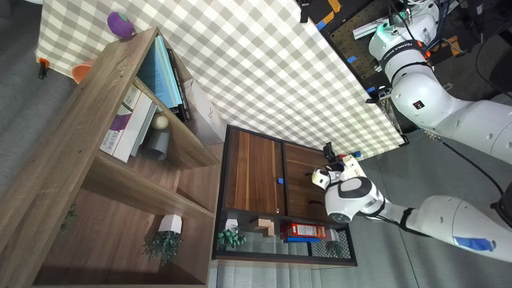
\includegraphics[width=0.23\textwidth]{figures/collage_of_envs/28.png} \\[-2pt]
    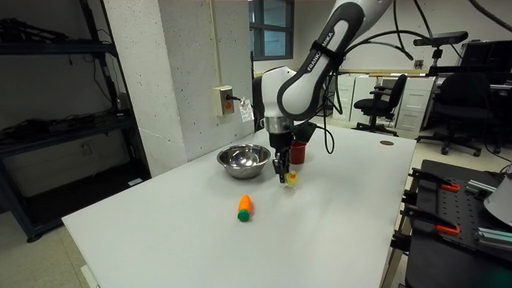
\includegraphics[width=0.23\textwidth]{figures/collage_of_envs/29.png} &
    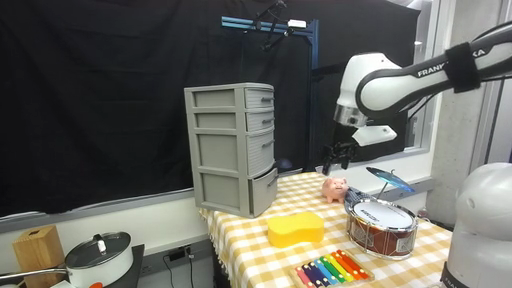
\includegraphics[width=0.23\textwidth]{figures/collage_of_envs/30.png} &
    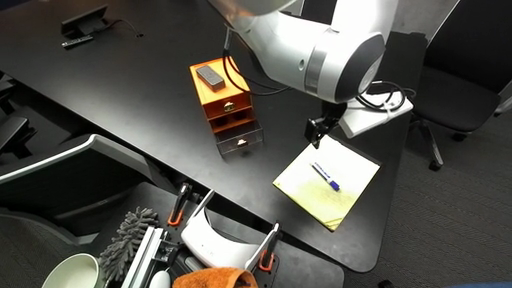
\includegraphics[width=0.23\textwidth]{figures/collage_of_envs/31.png} &
    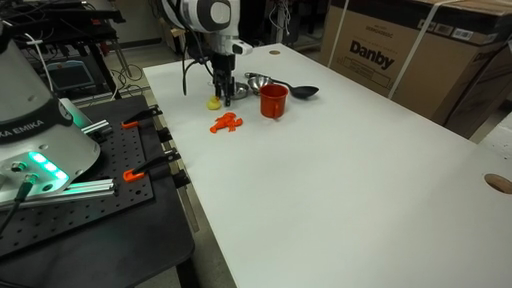
\includegraphics[width=0.23\textwidth]{figures/collage_of_envs/32.png}
  \end{tabular}
  \caption{Environments in RoboArena are diverse, due to RoboArena's distributed nature and the eschewing of a standardization of tasks. Here we depict 32 sample environments used for RoboArena across the network of participating institutions. Evaluators were encouraged to scale diversity, leading to a visible heterogeneity of environments. Even when the physical location of the robot was the same, lighting, camera viewpoints, tablecloths, and objects were often altered significantly, again made easy by the fact that exact scenes and tasks need not be standardized.}
  \label{env_collage}
\end{figure}

\section{Nuances in Policy Preference Labels}
\label{app:comp_over_progress}

Evaluators participating in the RoboArena evaluation framework are asked to provide a rough estimate of partial success of each rollout on the prescribed task, but also critically, a preference label specifying whether they liked policy A versus B on the same task. As we will outline here, this preference feedback can contain quite a bit of information beyond what is present in the partial success feedback. Concretely, figure~\ref{tab:pref_feedback_examples} depicts a few examples where \emph{partial success feedback was the same for policies A and B}, yet the evaluator marked a clear preference for either A or B.

\begin{table}[ht]
  \centering
  \caption{Examples of preference feedback for A/B pairs for which partial success feedback was equal for A and B, illustrating information beyond binary partial‐success scores.}
  \label{tab:pref_feedback_examples}
  \begin{tabular}{@{}ccp{0.73\textwidth}@{}}
    \toprule
    Session ID & Preferred Policy & Long‐form Feedback \\
    \midrule
    748 & A & Although both policies don’t put the cloth on the screwdriver, policy A places the cloth close to the banana, while policy B does not seem close to either object. \\
    674 & B & Both policies completed the entire task but policy B did it on the first try. After the first grasp and lift, it feels like policy A dropped the mouse prematurely. It then picked it up again and moved it further. \\
    660 & B & Policy B initially hesitated to move long distance but later transitioned to effective and rapid movements. Meanwhile, policy A also succeeded at the task, but it exhibited more sluggish movements. \\
    649 & A & Both A and B picked up the cup instead of pushing, and both then placed it on the table. After letting go, A returned to a starting pose while B kept repeatedly grabbing the cup, which is sub‐optimal. \\
    648 & B & While both did take the object out of the bowl (qualifying for full score), B placed the object on the table area next to the bowl. This is the more natural thing to do. \\
    641 & A & Both policy A and policy B almost solved the task completely. However, policy A displayed more decisive motions with less corrective behavior while policy B solved the task by chance after multiple attempts. \\
    579 & A & Both policies were able to close the drawer most of the way. However, policy A went straight for the drawer and didn’t stop until it was closed. Policy B got distracted by the plastic food items halfway through (though it eventually returned to close the drawer). \\
    \bottomrule
  \end{tabular}
\end{table}

We further found experimentally that for \textbf{11\%} of all A/B evaluations, the preference feedback did not agree with the partial success feedback, either because partial feedback was equal but the preference was not, or partial feedback and preference feedback displayed opposing trends. Thus, preference feedback is a uniquely rich data source for policy evaluations. 


\begin{figure}[H]
    \centering
    \includegraphics[width=\linewidth]{figures/strengths_weaknesses.pdf}
    \caption{We observe that policies tend to succeed on tasks involving direct object manipulation, such as placing objects into containers (examples in \textcolor{green}{green}), but often fail in tasks that require tool use or nuanced semantic understanding, such as wiping, cleaning or following detailed multi-step instructions (examples in \textcolor{red}{red}).}
    \label{figure:strengths_weaknesses}
\end{figure}

\section{Policy Performance Reports}
\label{app:performance_report}

To assist in the analysis, we use our automated pipeline to generate detailed reports that summarize the behavior and performance of each policy across a wide range of manipulation tasks based on data collected during distributed evaluation episodes. In the pipeline, we prompt OpenAI’s \texttt{o3-2025-04-16} model with the prompt template shown in \cref{figure:full_policy_performance_analysis_prompt} to automatically generate a structured policy performance report for a given policy. 
We include a representative full report for $\pi_0$-FAST-DROID in \cref{figure:pi0_fast_droid_full_performance_report} with the video references removed. 
 We further concisely summarize the resulting full report using the prompt in \cref{figure:summary_policy_performance_analysis_prompt}.
The reports for all evaluated policies \emph{with video references to specific evaluation episodes} are available at \href{https://robo-arena.github.io/leaderboard}{https://robo-arena.github.io/leaderboard}.

\section{Strengths and Weaknesses of the Evaluated Generalist Policies}
\label{app:policy_eval_summary}

To our knowledge, the evaluation done in this work is the most comprehensive evaluation of generalist policies to date. Analyzing the head-to-head comparisons across a diverse set of real-world tasks, we identify consistent behavioral patterns and failure modes exhibited by current policies. In this section, we synthesize the general strengths and weaknesses observed across all evaluated policies and the trends that emerge across policy families.

A primary strength of these generalist policies is their ability to operate in diverse viewpoints, lighting conditions, and background appearances. Across the evaluated policies, we observe that tasks involving direct object manipulation (e.g., pick-and-place, pushing, toppling, and simple open/close tasks) are more reliably solved than those requiring tool use, cloth manipulation or complex semantic understanding (\cref{figure:strengths_weaknesses}). In particular, these policies tend to perform better when goals are straightforward and visually grounded but struggle when the task demands precision alignment, multi-step reasoning or specific attribute perception like object class or color. Tasks involving deformable objects (e.g., folding, draping) and actions with tools (e.g., wiping, scooping) remain key challenges, often resulting in partial motion or outright frozen behavior. The weaknesses highlight the gaps in generalization, robustness, and physical interaction across various manipulation tasks.

When comparing the different policy families, autoregressive policies (e.g., PG-FAST-DROID, PG-FAST+-DROID, $\pi_0$-FAST-DROID) consistently achieve higher success rates in pick-and-place, stacking, and classification tasks, due to their more precise language following. Diffusion-based policies (e.g., PG-flow-DROID, $\pi_0$-flow-DROID) perform well in fluid or continuous motion tasks like sliding and wiping but often lag in tasks have precise language instructions (e.g., knocking over specific objects). Binning policies (e.g., PG-Bin-DROID) consistently underperform in nearly all tasks, with frequent inactivity and low task completion. Overall, substantial work remains to be done to achieve reliable and generalizable robot policies.




\begin{figure}[ht!]
\colorbox{gray!10}{
\begin{minipage}{\linewidth}
\fontsize{7pt}{8pt}\selectfont
1. Policy Overview \par
pi0\_fast\_droid is a fast, reactive manipulation policy that rarely idles and generally succeeds at single-object pick-and-place routines.  When the goal object is visually salient it plans a direct path, grasps confidently, and often retries after a failed grasp.  The policy copes reasonably well with mild clutter and can manipulate flexible objects such as towels or cloths.  Limitations become evident whenever the task demands fine tool control, accurate alignment (e.g., insertions or stacking), deliberate inaction, or multi-step reasoning.  In those settings the controller may oscillate, freeze, or grasp the wrong item, and it occasionally terminates without releasing the object it is holding. \par
\vspace{1em}
2. Comparative Performance (head-to-head)  \par
• Pick and Place – Across dozens of episodes pi0\_fast\_droid beat or tied the competing policy more often than it lost.  It routinely grasped the correct item and reached the target location, while rival policies either froze or mis-grasped (e.g., ducks into cups, cups into bowls, blocks into trays). \par
• Cover / Drape / Fold – The policy consistently outperformed its counterpart; it was usually the only agent to lift cloth or achieve partial folding, whereas competitors often merely poked at the fabric.  \par
• Sorting / Classification – In repeated colour-based sorting tasks pi0\_fast\_droid identified target colours correctly and placed them, while the alternative policies hesitated or selected wrong colours.  \par
• Move / Slide – When required to slide or reposition an object, the policy succeeded with smoother, faster trajectories; rival controllers tended to overshoot or stall. \par 
• Tool Use – Performance lagged behind the comparison agent: pi0\_fast\_droid lost or tied in most erasing, wiping, stirring or “clean the table” episodes, whereas the other policies executed smoother tool contact and fewer redundant motions.  \par
• Open / Close – The policy underperformed; it either failed to latch onto handles or to finish closing motions, while the competing agent completed the same drawer or cabinet tasks more reliably.  \par
• Object Manipulation – When asked to re-orient blocks, pour or open bottles, the policy frequently lost or tied; the competitor could align objects more precisely or at least avoid freezing.  \par
• Group / Organize / Stack – Stacking success was mixed; pi0\_fast\_droid often placed items near the correct spot but the rival policy achieved proper alignment more often, leading to several losses. \par
\vspace{1em}
3. Strengths  \par
• Robust grasping of familiar rigid objects; e.g., picked the cup and placed it into a basket smoothly, and removed a block from a box despite flaps in the way.  \par
• Re-attempt behaviour: after missing the bowl the first time it re-planned, re-grasped, and completed the pineapple placement.  \par
• Effective colour/shape recognition that supports sorting and non-red discrimination tasks.  \par
• Cloth manipulation: successfully folded a towel and achieved full coverage over a piggy-bank while the opponent merely poked.  \par
• Quick object search sweeps that cover shelves and table surfaces before freezing competitors, e.g., “find the creeper toy”. \par
\vspace{1em}
4. Weaknesses  \par
• Frequent freezing or limited exploration after one failed attempt, stalling entire episodes.  \par
• Tool control deficiencies: could not keep the eraser in contact with the board or open a water bottle despite grasping the cap.  \par
• Mis-identification of targets in clutter, e.g., placed tape in the wrong plate and grasped the robot instead of the marker meant to hit it.  \par
• Difficulty with precision insertions (portafilter into grinder, small cubes onto stacks) leading to losses.  \par
• Does not always release objects after placement, leaving grasped items hovering and tasks incomplete. \par
\vspace{1em}
5. Instruction Following  \par
• Handles colour and spatial qualifiers well (“blue cup into yellow bowl” succeeded). \par
• Fails at “do absolutely nothing” – still moved despite the explicit negation. \par
• Interprets minor typos (“non-read” → non-red) correctly and complied.  \par
• Multi-step or relational instructions are followed inconsistently; it dropped the towel but never folded it in “place carrot then fold towel”.  \par
• Occasionally ignores action verbs and grasps the wrong reference (picked the robot instead of using the marker to hit it). \par
\vspace{1em}
6. Reasoning  \par
Scene reasoning strengths: correctly inferred colour grouping goals and located all cups quickly in cluttered scenes.  \par
Weaknesses: often violates order constraints (tried to stack before tray placement) or stops after partial completion (emptied only one item then froze).  Spatial reasoning is sometimes coarse; the controller places objects “near” rather than “inside/on top”, leading to almost-correct states that still lose. \par
\vspace{1em}
7. Manipulation Skills \par
• Grasping: robust with medium-sized rigid objects (cups, blocks, towels).  \par
• Placing: accurate onto large, open targets; less precise for narrow targets or stacking (frequent mis-alignment of tape rolls).  \par
• Stacking/Inserting: partial success, but alignment errors common; blocks often dropped from height.  \par
• Tool manipulation: weak torque control when erasing, wiping or turning caps; slips off tools or hovers without making contact.  \par
• Recovery: will back-off and re-grasp after a miss instead of giving up.  \par
• Release: occasionally forgets to open gripper after placement. \par
\vspace{1em}
8. Robustness to Scene Variations  \par
• Handles moderate clutter and distractors, succeeding in busy kitchen and office scenes.  \par
• Cloth backgrounds, patterned tables, and partial occlusions rarely confuse its perception.  \par
• Sensitive to low-light episodes: performance degraded in dim “Place cup right side up” and “Put the yellow ducks in mug” scenes.  \par
• Wrist-camera occlusions sometimes cause it to mis-localise small targets (e.g., screwdriver into mug task). \par
\vspace{1em}
9. Common Failure Modes  \par
• Freezing after first error or mid-air hover with object still grasped. \par  
• Grasping the correct item but never releasing it into the goal.  \par
• Selecting a distractor of similar colour/shape (tape vs. stapler, carrot vs. duck). \par  
• Over-shooting and colliding with cabinets or shelving.  \par
• Tool tasks: pushes or nudges the tool instead of forming a stable grasp, leading to repeated but ineffective motions.  \par
• Misinterpreting passive, negated, or multi-step instructions (moved during “do not move”, folded towel step omitted, etc.). \par
\vspace{1em}
Overall, pi0\_fast\_droid provides a solid baseline for everyday pick-and-place and cloth-handling tasks, but would benefit from improved tool manipulation control, tighter release logic, and more deliberate high-level planning for multi-step or precision-alignment scenarios.
\end{minipage}
}
\caption{The full generated policy performance report for $\pi_0$-FAST-DROID (video references removed; check \href{https://robo-arena.github.io/leaderboard}{https://robo-arena.github.io/leaderboard} for interactive reports with references).}
\label{figure:pi0_fast_droid_full_performance_report}
\end{figure}


\begin{figure}[ht!]
\colorbox{gray!10}{
\begin{minipage}{\linewidth}
\fontsize{8pt}{8pt}\selectfont
We are evaluating a policy named \texttt{POLICY NAME} deployed on a robot arm to perform various manipulation tasks.\par
This policy was compared head-to-head against other policies across multiple episodes. Each episode includes:\par
\begin{itemize}
    \item A session ID
    \item A task description and the task category it belongs to. The possible task categories are: Pick and Place, Open / Close, Move / Slide, Knock Over / Topple, Cover / Drape / Fold, Group / Organize / Stack, Find / Search, Minimal or No Action, Object Manipulation, Sorting / Classification, Tool Use.
    \item A scene and task analysis
    \item Head-to-head evaluation results
\end{itemize}

Using the episode data provided, generate a \textbf{structured and comprehensive summary report} in the format below:\par
\vspace{1em}
1. \textbf{Policy Overview}\par
A brief paragraph summarizing the general behavior, capabilities, and limitations of the policy.\par
\vspace{1em}
2. \textbf{Comparative Performance}\par
How the policy performed in head-to-head comparisons against other policies across the different task categories. For each task category, create a bullet point with a discussion of how the policy consistently outperformed or underperformed compared to all the other policies. Make sure in this section that every claim about the policy is with respect to other competing policies. When making a claim, always mention how the other policies performed in comparison to the current policy. Do not discuss the policy in isolation. Don't mention a task category unless there is evidence of the policy performing well or poorly in that category across multiple episodes. Make your claims based on overall performance or underperformance for specific task categories rather than individual episodes. There is no need to reference specific session IDs in this section (no \texttt{<ref>} tags).\par
\vspace{1em}
3. \textbf{Strengths}\par
Bullet-pointed list of notable strengths in manipulation behavior or general reliability. Mention the task categories the policy is good at (if any) instead of basing a claim on a single instance. Focus on generalizable behaviors like smooth trajectories, robust grasping, or adaptability. Use concrete examples and session ID citations.\par
\vspace{1em}
4. \textbf{Weaknesses}\par
Bullet-pointed list of recurring limitations or error patterns. Mention the task categories the policy is poor at instead of basing a claim on a single instance. Mention issues such as fine motor control, object confusion, multi-step failure, etc. Include session ID references with \texttt{<ref>} tags.\par
\vspace{1em}
5. \textbf{Instruction Following}\par
Analyze how well the policy understands and executes task instructions. Note sensitivity to language structure, ability to follow negated or relational commands, issues with ambiguous phrasing, ability to handle typos, etc. Cite session-specific evidence.\par
\vspace{1em}
6. \textbf{Reasoning}\par
Evaluate the policy's ability to reason about both the \textbf{scene context} (e.g., spatial relationships, object visibility) and the \textbf{text instruction} (e.g., goal inference, conditional logic). Mention cases where reasoning appears strong or deficient. Use \texttt{<ref>} tags to support your analysis.\par
\vspace{1em}
7. \textbf{Manipulation Skills}\par
Describe the physical performance of the policy: grasping, placing, stacking, inserting, pouring, drawer use, and recovery from errors. Use examples to show when skills succeed or fail.\par
\vspace{1em}
8. \textbf{Robustness to Scene Variations}\par
Assess the policy's performance under different lighting, clutter levels, object positions, and camera views. Note any sensitivities to occlusion or distractors, etc.\par
\vspace{1em}
9. \textbf{Common Failure Modes}\par
List frequently observed failures (e.g., freezing mid-task, grabbing wrong item, failing passive commands). Provide short descriptions and supporting citations.\par
\vspace{1em}
\textbf{Instructions:}\par
\begin{itemize}
    \item When referring to a session, always cite the full session ID (UUID format, e.g., \texttt{16e5bbda-57c1-4e58-a24a-b39ee8142d41}) exactly as provided. Do not shorten, truncate or modify it in any way.
    \item Always wrap session IDs inside \texttt{<ref>...\texttt{</ref>}} tags. Example: \texttt{<ref>16e5bbda-57c1-4e58-a24a-b39ee8142d41</ref>}
    \item Try to cite as many session IDs as possible to support your claims, but only if they are relevant to the point you're making.
    \item Avoid generalizing from a single episode unless there is clear evidence of a pattern.
    \item Keep the tone analytical and professional, emphasizing repeatable behaviors and insights.
    \item Do not invent session IDs. Only use session IDs present in the provided episode reports.
    \item There is no need to mention the specific number of episodes and wins/losses/ties in head-to-head evaluations in this report.
\end{itemize}

\vspace{1em}
The individual episode reports are as follows:\par
\vspace{1em}
\texttt{========== Episode Report \#1 ==========}\par
...
\end{minipage}}
\caption{The prompt template used to generate the full policy performance reports.}
\label{figure:full_policy_performance_analysis_prompt}
\end{figure}


\begin{figure}[ht!]
\colorbox{gray!10}{
\begin{minipage}{\linewidth}
\fontsize{8pt}{9pt}\selectfont
Given the following full evaluation report of a robot manipulation policy, generate a concise, high-quality summary that captures the main findings from sections 1 through 9.\par

\vspace{1em}
Each bullet should summarize the corresponding section in a few sentence fragments, focusing on the most important points. Avoid excessive detail, ensure clarity and correctness. Stick to the facts presented in the full report.\par

\vspace{1em}
Use the following format exactly:\par

\vspace{1em}
- Policy Overview: \textless{}summary\textgreater{}\par

\vspace{1em}
- Comparative Performance: \textless{}summary\textgreater{}\par

\vspace{1em}
- Strengths: \textless{}summary\textgreater{}\par

\vspace{1em}
- Weaknesses: \textless{}summary\textgreater{}\par

\vspace{1em}
- Instruction Following: \textless{}summary\textgreater{}\par

\vspace{1em}
- Reasoning: \textless{}summary\textgreater{}\par

\vspace{1em}
- Manipulation Skills: \textless{}summary\textgreater{}\par

\vspace{1em}
- Robustness to Scene Variations: \textless{}summary\textgreater{}\par

\vspace{1em}
- Common Failure Modes: \textless{}summary\textgreater{}\par

\vspace{1em}
Place a line break between each bullet point. Don't output anything before or after the bullet points.\par

\vspace{1em}
Here is the full report to summarize:\par

\vspace{1em}
\texttt{FULL REPORT}\par
\end{minipage}}
\caption{The prompt template used to generate a concise summary of the full policy performance report.}
\label{figure:summary_policy_performance_analysis_prompt}
\end{figure}
